% !TEX TS?program = pdflatexmk
\documentclass{article}
\usepackage{geometry}
\usepackage{amsmath}
\usepackage{amssymb}
\usepackage{bold-extra}
\usepackage{authblk}
\usepackage[backend=biber, citestyle=authoryear]{biblatex}
\usepackage{graphicx}
\usepackage{epstopdf}
\usepackage{placeins}
\usepackage[width=.8\linewidth, labelfont=bf]{caption}
\usepackage[
	hidelinks,
	colorlinks=true,
	allcolors=blue
]{hyperref}

\addbibresource{bibliography.bib}
\graphicspath{{.}}

\setlength{\parindent}{0em}
\setlength{\parskip}{0.25cm}
\geometry{
	a4paper,
	left=1in,
	right=1in,
	top=0.75in,
	bottom=0.75in
}

\title{\sc COVID-19 Age-Structured SEIR Model\\\Huge{\bfseries Technical Report}} %FIXME
\author[1]{Pranav Minasandra}
\author[2]{Vishwesha Guttal}
%\author[3]{Prateek Sharma}
%\author[4]{Shivkumar Jolad}
%
\affil[1]{Centre for Ecological Sciences \& UG Programme,  Indian Institute of Science, Bengaluru}
\affil[2]{Centre for Ecological Sciences,  Indian Institute of Science, Bengaluru}
%\affil[3]{Department of Physics, Indian Institute of Science}
%\affil[4]{Public Policy, School of Liberal Education, FLAME University, Pune}
\date{}

\begin{document}
\maketitle\hrule

\section*{Disclaimer}
This model is simple, ignores many features of real disease dynamics and demographic features of Indian population. Hence, it is to be used only for understanding concepts but NOT for making quantitative forecasts about the pandemic. 
%
%\section{What is this model?}
%This is an age-structured SEIR compartmental model of the epidemiology of the coronavirus that causes COVID-19.
%
%Here, we assume, with respect to the disease, that all individuals can be categorised as one of the following:
%\begin{itemize}
%\item Susceptible ($S$)
%\item Exposed ($E$) (to virus but not sick yet)
%\item Infectious ($I$) (who in turn are categorised into asymptomatic, symptomatic (mild-moderate), hospitalised and critically ill). 
%\item Recovered  ($R$)  (and hence immune)
%\item Dead ($D$)
%\end{itemize}
%
%\emph{Age-structured} means is that we account for the age structure of a particular demographic. In our specific case, we pay attention to what proportion of the population is senior citizens.
%
%This model is parametrised for the states of Maharashtra, Karnataka, Tamil Nadu, and the country of India. The parameters were derived from intelligent guesswork from multiple data sources (see the About section, but also Caveats).
%
%\section{What is the use of this model?}
%This model can be used to understand how the epidemic spreads without and with interventions. Specifically, we incorporate two types of interventions -- one where the vulnerable population is isolated and the other is the complete lockdown. Therefore, we can investigate how different types of physical distancing and their effectiveness affects disease spread. 
%
%On Tab 2 (Total Infections), one can view the total number of individuals who have been affected by the virus. This can be seen for two different intervention conditions and a baseline sceario. 
%
%The model illustrates the role of incubation time, which provides the disease a sort of \emph{inertia}.
%
%On Tab 3 (Hospitalisations), we show the number of hospitalised individuals - based on our model analysis. There is a gap between when a person gets infected and when she/he is brought to a hospital; therefore, we see that this number reacts slowly to a lockdown. This effect could be seen in reality as well.
%
%\section{Can I plan according to the results of this model?}
%No. This model is for illustrative purposes only, and should not be used for quantitative forecasting.
%%Most models in this time will not be reliable, for the simple reason that not much is known about COVID-19 precisely.
%%Please wait for better parametrised more elaborate models that will surely appear at some point in the future.
%
%\section{Can I play with the code for this model?}
%Yes, please. The code for this model is available at our github repository:  
%If you have any questions regarding the modelling approaches used, please send a well-drafted email to
%\texttt{pranavm@iisc.ac.in} .
%
%\section{Why don't you show actually observed data anywhere?}
%Empirical data is subject to the dynamics of societal awareness of the disease, testing rates, stochasticity, and other numbers.
%Numerous questions have been raised about the data we have.
%Therefore, showing data in our plots could have been misleading.
%Moveover, there are many online sources where real data are beautifully shown. 
%We therefore refrain from showing this data. 
%
%%\section{Why don't you talk about the number of deaths?}
%%Our model incorporates this data, but we believe discussing this variable with models like these is irresponsible at a time like this.
%
%\section{Can you tell me more about your model?}
\section{Age-structured mathematical model for COVID-19}
Our population model is based on the classic SEIR models, which have been appropriately modified to include 
various epidemiological features of COVID-19. 
Our model closely follows the work of \cite{weitz2020} who has applied it to the US state Georgia, and was inspired by a simpler version by \cite{hill2020}. 

We assume that the population consists of susceptible ($S$), exposed ($E$), infected but asymptotic ($I_a$),  infected with mild symptoms ($I_s$),  infected requiring hospitalisation ($I_h$), infected and critical ($I_c$), recovered ($R$) and dead ($D$) individuals. The total population is given by $N=S+E+I_a+I_s+I_h+I_c+R+D$.

We incorporate some key empirical features of covid-19: (i) asymptomatic individuals can infect the susceptible (\cite{li2020science,park2020}) 
(ii) a person can recover directly from any of the infected stages, or progress sequentially towards higher severity and eventually death. 
(iii) Crucially, it is now well established that COVID-19 mortality rates are highly age-dependent, with the population of senior citizens who are 
vulnerable (aged more than 60 years) at substantially higher risk than the the younger population (those less than 60 years). Therefore, we incorporate the age-structure available for each of the (three)Indian states that we apply our model to. We consider two age-structures; we denote them as $S_1$ and $S_2$, representing younger and older populations, respectively. 

For each age-structure $S_i \,\, i \in \{1,2\}$, the dynamics of epidemic is given by:

\begin{align}
\dot{S_i} & = - \sum_j \frac{(\beta_{a,ji} I_{a,j} + \beta_{s,ji} I_{s,j} +  \beta_{h,ji} I_{h,j} + \beta_{c,ji} I_{c,j})}{N} S_i \\
\dot{E_i} & = \sum_j \frac{(\beta_{a,ji} I_{a,ji} + \beta_{s,ji} I_{s,j} +  \beta_{h,ji} I_{h,j} + \beta_{c,j} I_{c,i})}{N} S_i - \alpha_{e,i} E_i \\
\dot{I_{a,i}} & = (1-p_i) \alpha_{e_i} E - \gamma_{a,i} I_{a,i} \\
\dot{I_{s,i}} & =  p_i \alpha_{e,i} E   - \gamma_{s,i} I_{s,i} -  \alpha_{s,i} I_{s,i} \\
\dot{I_{h,i}} & =  \alpha_{s,i}  I_{s,i} -  \gamma_{h,i} I_{h,i}  -\alpha_{h,i} I_{h,i}  \\
\dot{I_{c,i}} & =  \alpha_{h,i} I_{h,i} - \gamma_{c,i} I_{c,i}  - \alpha_{c,i} I_{c,i}\\
\dot{R_i} & = \gamma_{a,i} I_{a,i} +  \gamma_{s,i} I_{s,i} + \gamma_{h,i} I_{h,i} + \gamma_{c,i} I_{c,i} \\
\dot{D_i} & =  \alpha_{c,i} l_{c,i} 
\end{align}

\noindent where $\beta_{x,ji}$'s represent transmission rate of infection from $j$ age-class to $i$ age-class from different infected groups $x$ (with $x \in \{a, s, h, c\}$),  $\gamma$'s represent the rate of recovery for different infected stages and $\alpha$'s represent the rate of progression from one stage of disease to the next. 

The dynamics of this model are shown in Fig.\ \ref{fig:modeldynamics}.
\begin{figure}
\centering
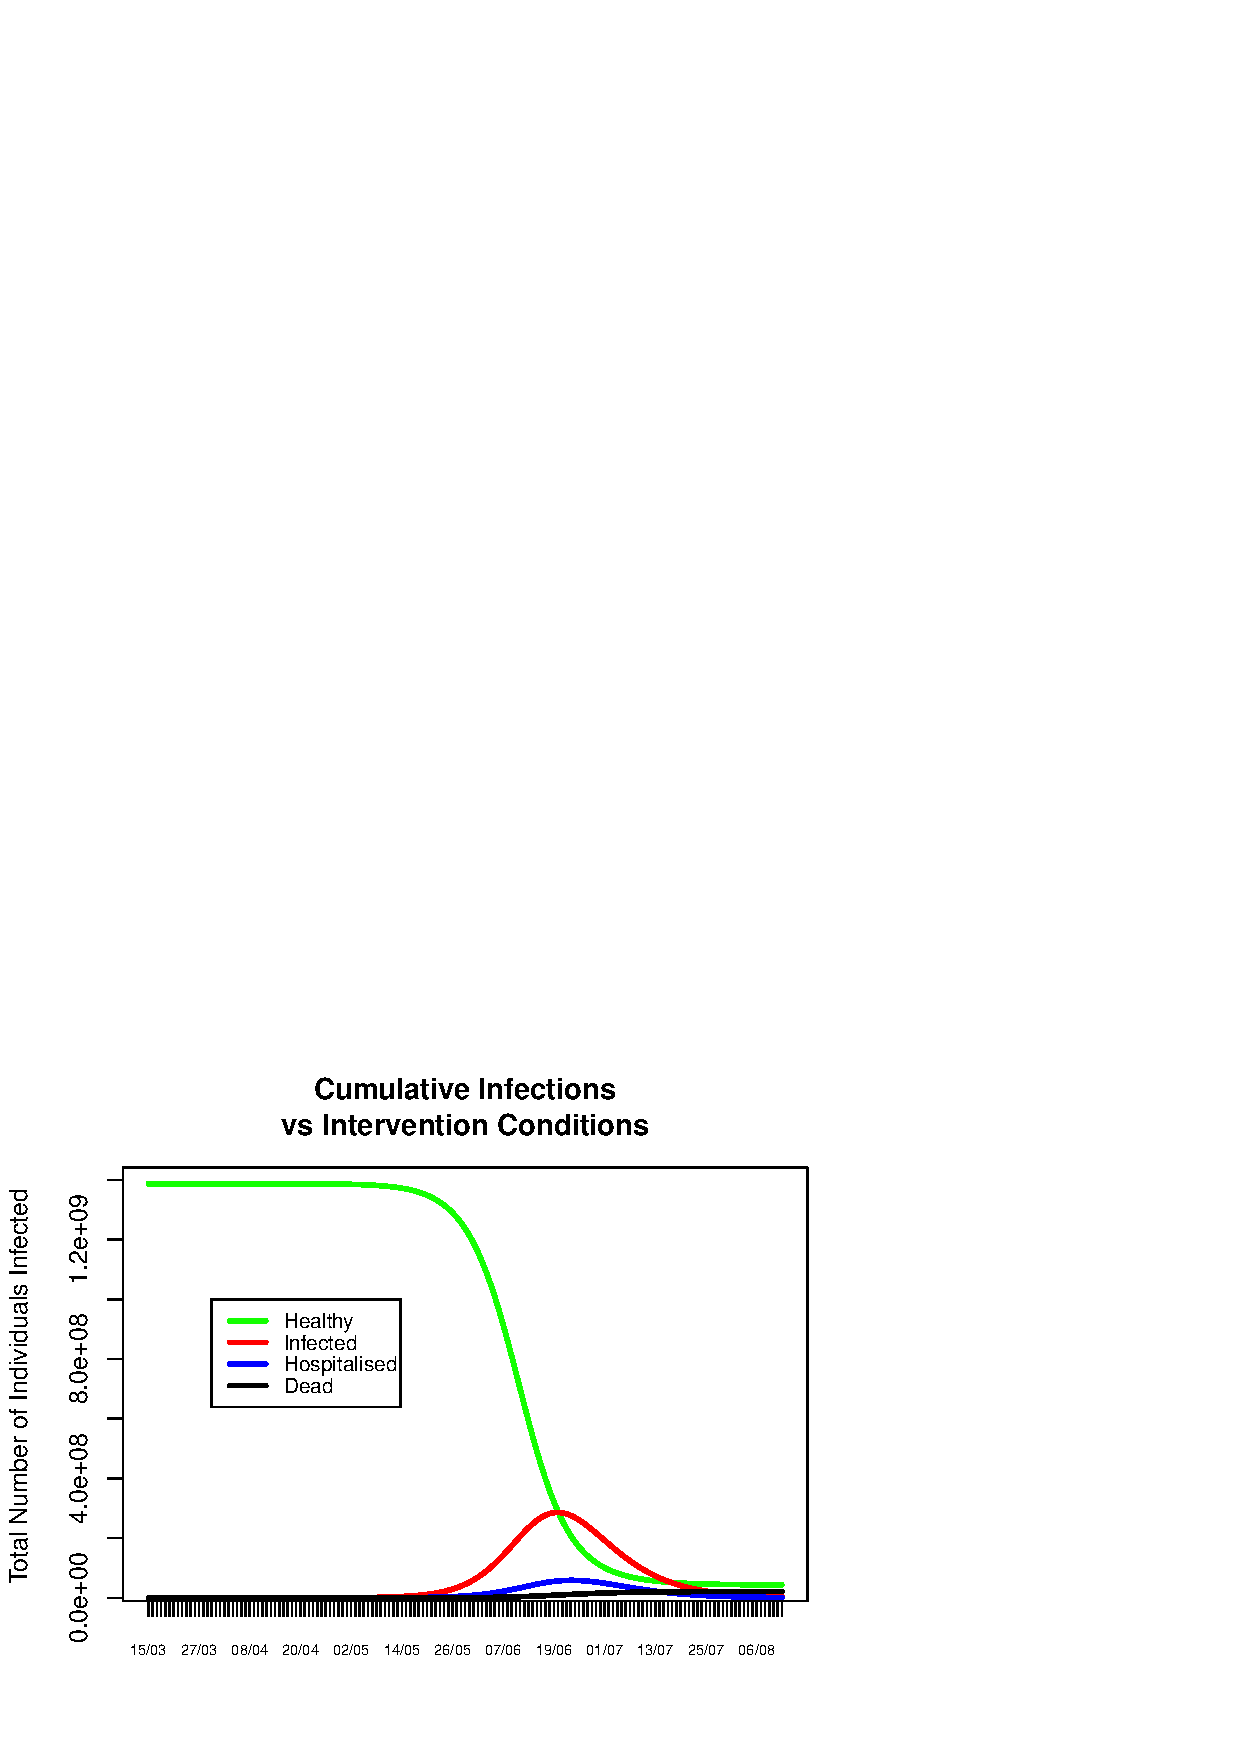
\includegraphics[width=.8\linewidth]{modeldynamics.png}
\caption{The typical dynamics of the COVID-19 pandemic, as expected by our model and parametrisation, are shown here.}
\label{fig:modeldynamics}
\end{figure}

\subsection{Model parameters}
We parametrise the model based on findings from recent studies (\cite{wu2020lancet,li2020science,park2020,hill2020}).  In Table 1, we list various epidemiological parameters from the literature. In general, we assume that older age-class is more likely to pass on to severe stages of the infection; we assume that this rate is twice that of the younger age group. We assume a high-mortality rate of the critically infected. See Table 2 for model parameters and Table 3 for relationship between model parameters and empirical values.

We incorporate the total population size and age-structure data for different states based on a model projection of population pyramid for 2021 which uses data from census-2011 of the government of India. See Tables 4. 

We consider three scenarios: 

(A) {\it Baseline scenario} - which assumes that the trends of the data from the first case in the state $24^{th}$ March 2020 will continue without a full lockdown. Therefore, this baseline includes various measures in place in India upto $24^{th}$ March 20120, such as contact tracing, home quarantine of the suspected, hospital quarantine of the positive cases, etc. Here, we assume that rate of infection of the susceptible population does not depend on age structure; this is motivated by the recent analyses by \cite{singh2020} which shows that house-holds in India often have three-generational interactions.

(B) {\it Lockdown}: We then consider the impact of lockdown which was initiated on $25^{th}$ March. Here, since the rate of effectiveness of such a lockdown is difficult to quantify, especially in light of the migrant population movement it triggered and an in-general denser population profile of India,  we consider two scenarios -- a moderate reduction of the transmission rates (in particular $\beta_a$ and $\beta_s$) corresponding to 75\% or a partial success of $50\%$ only.

(C) {\it Protect the vulnerable}: Here, in addition to the restrictions in baseline scenario, the priority given to protect the vulnerable -- who are typically aged and/or have comordibities like diabetes, hypertension, cardiac or respiratory problems. Therefore, we set only some $\beta$'s to low values. Note that this measure will protect transmission of disease from asymptomatic younger population to the old, but not among younger populations. Specifically, we assume the following transmission rates for asymptomatic individuals:$\beta_{a,12} = 0.25 \beta_a$, $\beta_{a,22}=0.25 \beta_a$, $\beta_{a,11} = \beta_{a,21} = \beta_a$. For the symptomatic, we assume $\beta_{s,12} = 0.1 \beta_s$, $\beta_{s,22}=0.1 \beta_s$, $\beta_{s,11} = \beta_{s,21} = \beta_s$. 

Various intervention measures can reduce the damage caused by the pandemic to varying extents.
Figs.\ \ref{fig:infs}, \ref{fig:hosps}, and \ref{fig:deaths}  show how much each intervention measure can affect the dynamic if applied indefinitely.
It is clear that the lockdown is most likely a very strong measure to control the disease,
but (a) it is not possible to know the strength of the lockdown accurately, and (b) an indefinite
lockdown is not feasible for various reasons. In the app, you can control the duration and strength of the lockdown, and 
examine qualitatively the effects it can have on pandemic spread.

\begin{figure}[htp]
\centering
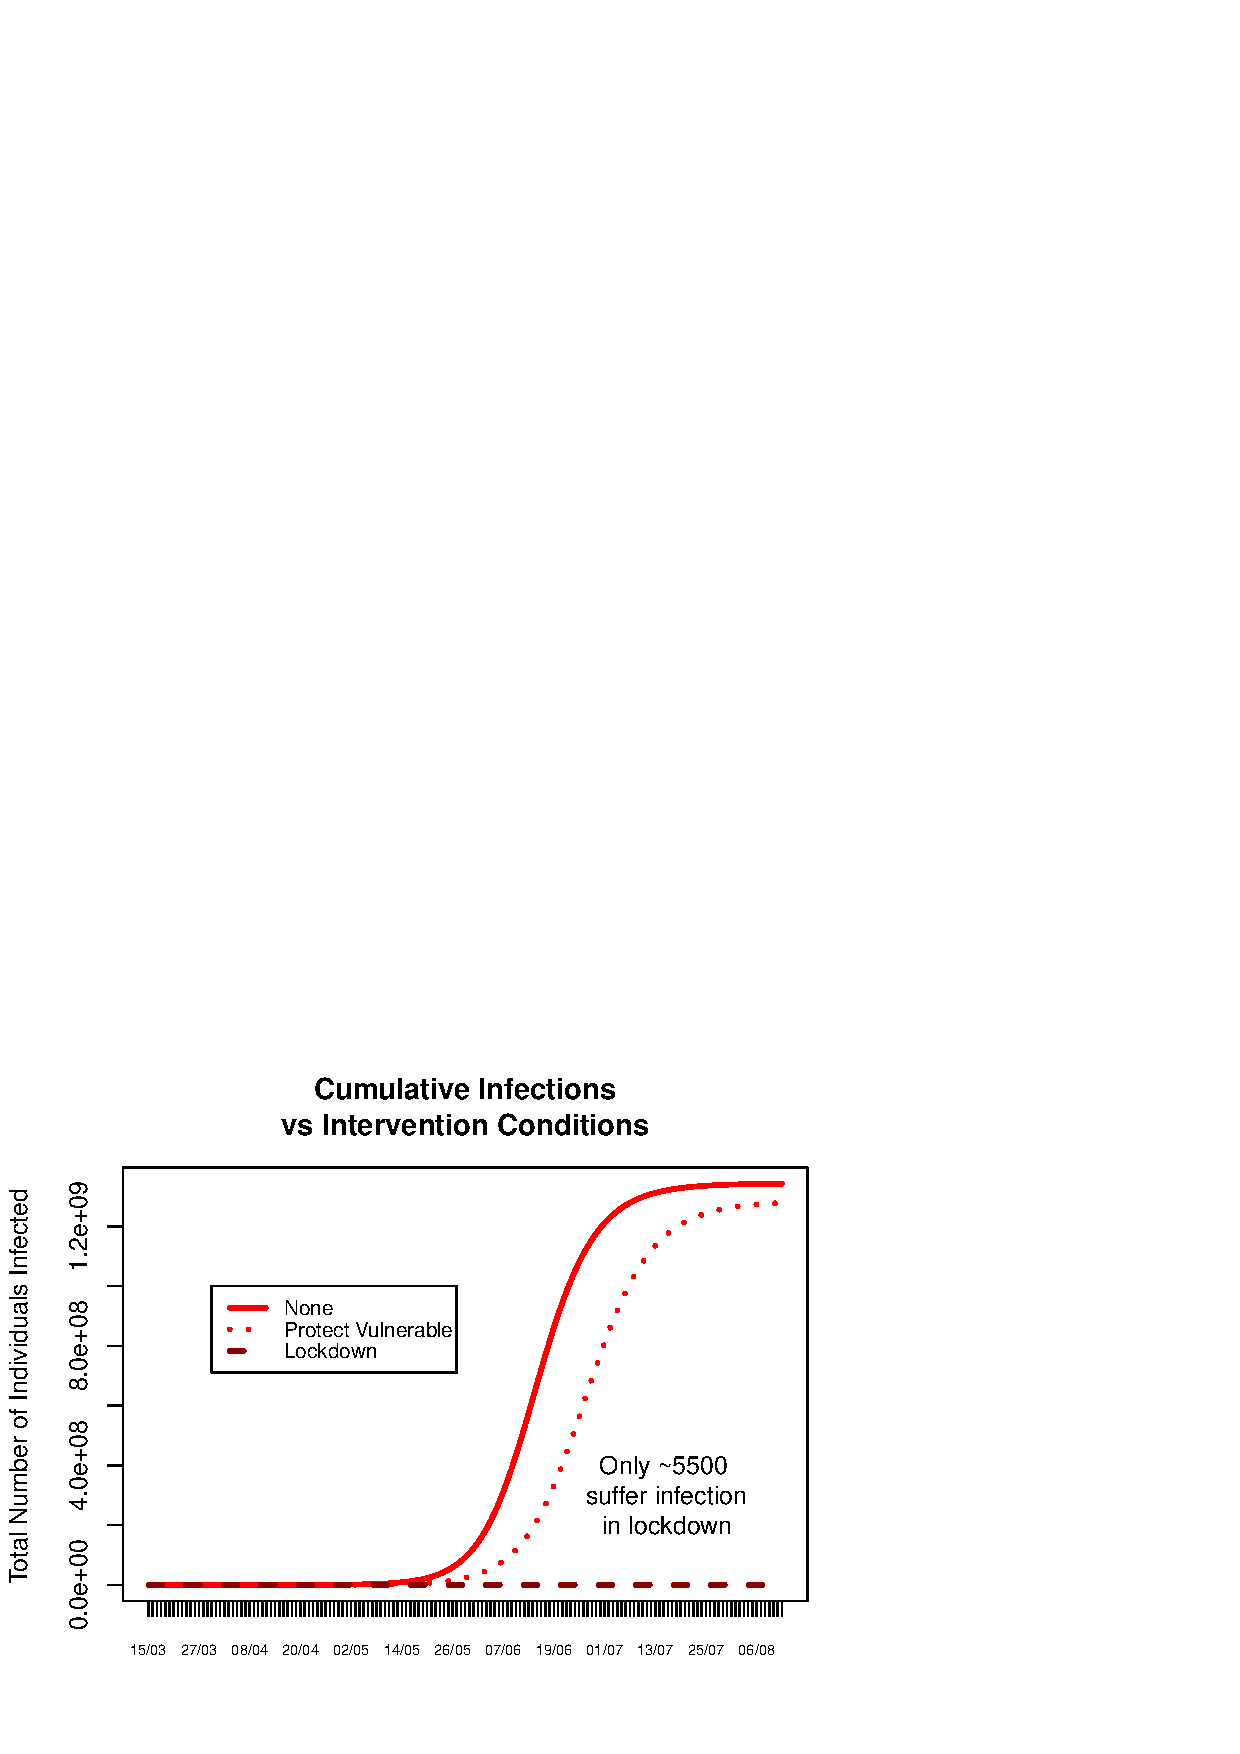
\includegraphics[width=.8\linewidth]{infsvsint.png}
\caption{Infections in the COVID-19 pandemic as functions of time, as expected by our model and parametrisation, are shown here.}
\label{fig:infs}
\end{figure}
\begin{figure}[htp]
\centering
\includegraphics[width=.8\linewidth]{hospvsint.png}
\caption{The numbers of hospitalised individuals, as expected by our model and parametrisation, are shown here.}
\label{fig:hosps}
\end{figure}
\begin{figure}[htp]
\centering
\includegraphics[width=.8\linewidth]{deathsvsints.png}
\caption{The number of deaths predicted by our model and parametrisation, are shown here.}
\label{fig:deaths}
\end{figure}

Age-structuring of a population can have impact on the deaths caused by this pandemic.
Fig. \ref{fig:age} shows how hypothetical populations with different numbers of senior citizens 
can react very differently to a pandemic. We very cautiously predict that India might have a lower
overall COVID-19 death rate than other countries owing to its relatively younger population.
However, due to large population sizes in India, the absolute number of deaths might be higher.

\begin{figure}
\centering
\includegraphics[width=.8\linewidth]{effectsofage.png}
\caption{Here, 3 hypothetical populations with 1000 individuals each is attacked by the COVID-19 pandemic.
	Death rates as functions of age-structure are shown.}
\label{fig:age}
\end{figure}

\FloatBarrier
\begin{table}[htp]
\caption{Empirical parameters}
\begin{center}
\begin{tabular}{|c|c|c|}
\hline
Term & Description & Value  						 \\  \hline
$\tau_I$ & Average incubation period & 5 days 				 \\
$\tau_a$ & Average duration of asymptomatic infections & 7 days 	 \\ 
$\tau_s$ & Average duration of mild symptomatic infections & 7 days 	 \\
$\tau_h$ & Average duration of hospitalisations & 4 days 		 \\
$\tau_c$ & Average duration of ICU admissions & 10 days 		 \\
$p_a$ & Fraction of asymptomatic cases & 0.3 				 \\
$p_s$ & Fraction of mild symptomatic cases & 0.55 			 \\
$p_h$ & Fraction of hospitalisations & 0.15 				 \\
$p_c$ & Fraction of severe cases & 0.05 				 \\
$f_c$ & Case fatality rate & 0.01 					 \\
\hline
\end{tabular}
\end{center}
\label{basic-seir:params}
\end{table}%

\begin{table}[htp]
\caption{Model parameter definitions and their values}
\begin{center}
\begin{tabular}{|c|c|c|}
\hline
Parameter & Description & Value \\ \hline
$\beta_{a,ji} = \beta_a$ & Transmission rate from asymptomatic individuals to susceptible  & 0.3 per day \\
$\beta_{s,ji} = \beta_s$ & Transmission rate from symptomatic individuals & 0.6 per day \\
$\beta_{h,ji} = \beta_h$ & Transmission rate from hospitalised individuals & 0.001 per day \\
$\beta_{c,ji} = \beta_c$ & Transmission rate from critical individuals & 0.001 per day \\
$p$ & Fraction of exposed who become symptomatic & 0.75 \\
$\gamma_{e,i} = \gamma_e$ & rate at which exposed individuals turn infected & $(\tau_I)^{-1}$ \\
$\gamma_{a,i} = \gamma_a$ & rate at which asymptomatic individuals recover & $(\tau_a)^{-1}$   \\
$\gamma_{s,i} = \gamma_s$ & rate at which symptomatic individuals recover & $p_s / \tau_s$ \\
$\alpha_{s,1}$ & rate at which young symptomatic individuals need hospitalisation &  $1/\tau_s - \gamma_s$ \\
$\alpha_{s,2}$ & rate at which old symptomatic individuals need hospitalisation &  $2\alpha_{s,1}$ \\
$\alpha_{h,1}$ & rate at which young hospitalised individuals become critical & $(\tau_h)^{-1} \, p_h /(p_h + p_c)$  \\
$\alpha_{h,2}$ & rate at which old hospitalised individuals become critical & $ 2 \alpha_{h,1}$ \\
$\gamma_{h,i}$ & rate at which hospitalised individuals recover &  $1/\tau_h - \alpha_{h,i}$ \\
$\alpha_{c,1}$ & rate at which young critical individuals die & $(\tau_c)^{-1} f_c / p_c $ \\
$\alpha_{c,2}$ & rate at which old critical individuals die & $2 \alpha_{c,1}$ \\
$\gamma_{c,i}$ & rate at which critical individuals recover &  $ 1/\tau_c - \alpha_{c,i}$  \\
\hline
\end{tabular}
\end{center}
\label{basic-seir:params}
\end{table}%

\begin{table}[htp]
\caption{Relationship between empirical and model parameters}
\begin{center}
\begin{tabular}{|c|c|c|}
\hline
Average incubation time & $\tau_a = 1/\gamma_e$  & \\ \hline
Duration of mild symptomatic cases & $\tau_s = 1/(\gamma_s+\alpha_s)$  &  $\alpha_s = 1/\tau_s - \gamma_s$ \\
Fraction of mild symptomatic cases & $ p_s=\gamma_s / (\gamma_s + \alpha_s) = \gamma_s \tau_s $ & $\gamma_s = p_s / \tau_s$  \\  \hline
Duration of hospitalisation & $\tau_h = 1/(\gamma_h + \alpha_h)$  &  $\gamma_h = 1/\tau_h - \alpha_h$  \\
Fraction of hospitalisations \& critical cases &  $ p_c /(p_h + p_c) = \alpha_h / (\gamma_h + \alpha_h)  = \alpha_h \tau_h $  &  $\alpha_h = (\tau_h)^{-1} \, p_h /(p_h + p_c)$  \\  \hline
Duration of critical cases & $\tau_c = 1/(\gamma_c + \alpha_c)$ &   $\gamma_c = 1/\tau_c - \alpha_c$ \\
Fraction of severe cases &  $ f_c / p_c =  \alpha_c / (\alpha_c + \gamma_c) = \alpha_c \tau_c $  & $\alpha_c = (\tau_c)^{-1} f_c / p_c $\\
\hline
\end{tabular}
\end{center}
\label{basic-seir:params}
\end{table}%
  
\begin{table}[htp]
\caption{Age-structure data of different states based on model projections for 2021. The fractions have been rounded off to nearest second decimal place}
\begin{center}
\begin{tabular}{|c|c|c|c|}
\hline
State & Total population & Upto 60 years  & Above 60 years\\  \hline
Maharashtra & 11.9 crores  & 0.89 & 0.11\\
Kerala & 3.45 crores & 0.86 & 0.14 \\
Karnataka  & 6.56 crores & 0.9 & 0.1\\
Tamil Nadu & 7.52 crores & 0.88 & 0.12 \\ \hline
All-of-India & 133 crores & 0.91 & 0.09 \\
\hline
\end{tabular}
\end{center}
\label{age-str}
\end{table}

\FloatBarrier\printbibliography
\end{document}
